\documentclass{article}
\usepackage{graphicx}
\graphicspath{ {images/} }

\title{The Book of Special Relativity}
\date{May 17th, 2017}
\author{Sishaar Rao}

\begin{document}
\pagenumbering{gobble}
\maketitle
\newpage
\pagenumbering{arabic}

Special relativity is a theory proposed by Albert Einstein that describes the propagation of matter and light at high speeds. It was invented to explain the observed behavior of electric and magnetic fields, which it beautifully reconciles into a single so-called electromagnetic field, and also to resolve a number of paradoxes that arise when considering travel at large speeds. Special relativity also explains the behavior of fast-traveling particle, including the fact that fast-traveling unstable particles appear to decay slower than identical particles traveling slower. Special relativity is an indispensable tool of modern physics, and its predictions have been experimentally tested time and time again without any discrepancies turning up. Special relativity reduces to Newtonian mechanics in the limit of small speeds.

\vspace{5mm}

According to special relativity, no wave or particle may travel at a speed greater than the speed of light c. Therefore, the usual rules from Newtonian mechanics do not apply when adding velocities that are large enough. For example, if a particle travels at a speed \( v \) with respect to a stationary observer, and another particle travels at a speed \( v' \)  with respect to the first particle, the speed \( u \) of particle two seen by the observer is not  as would be the case in Newtonian mechanics, but rather
\[
  u = \frac{v + v'}{1 + \frac{vv'}{c^2}}
\]

\newpage
\section{Invariance of Length’s Measured Perpendicular to Relative Motion}

\begin{figure}[!htb]
  \centering
  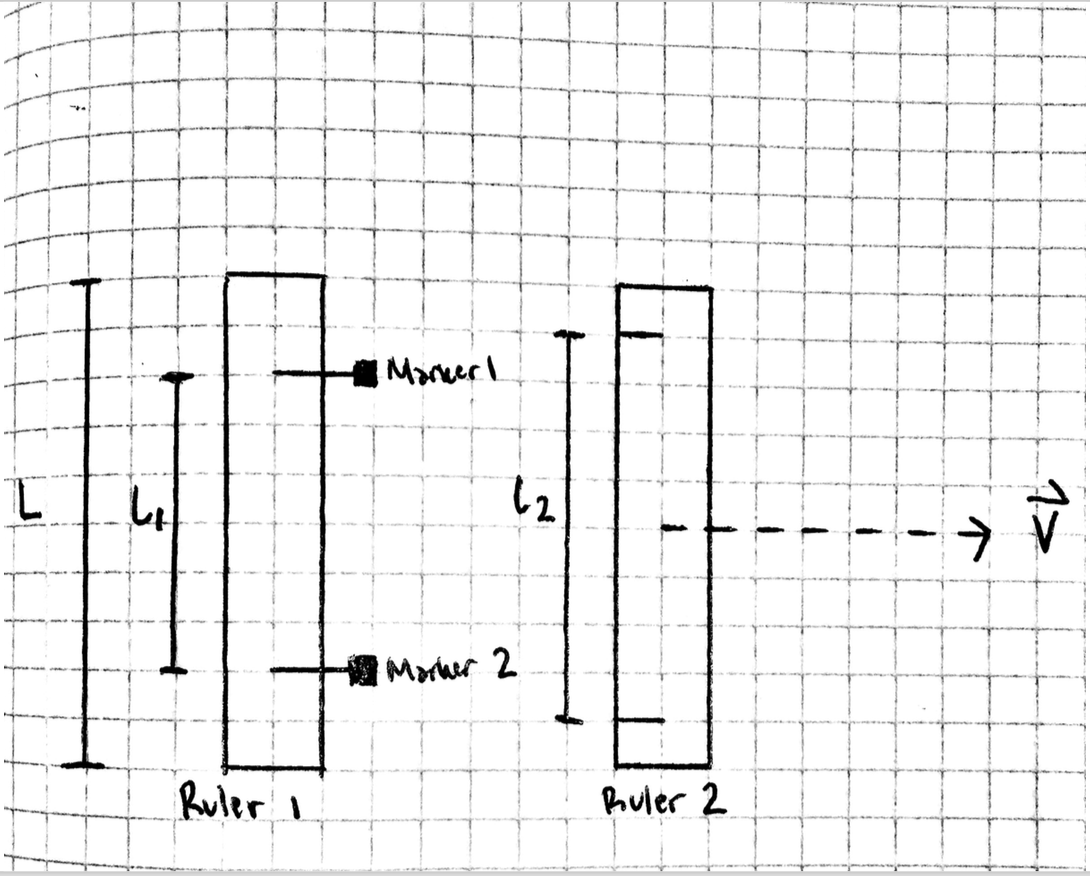
\includegraphics[width=100mm]{sticks}\par
  \caption{Two rulers perpendicularly flying past eachother}
\end{figure}

In the figure above, we are presented with a thought experiment:

\vspace{2mm}

Suppose we are given two rulers, Ruler 1 and Ruler 2 of length \(L\). Ruler 1 has two markers attached on it with a separation of \(L_1\). Our hypothesis is that if Ruler 2 is flying perpendicularly by Ruler 1 with a speed \(\vec{v}\), then Ruler 2 will become shorter than Ruler 1.

If indeed Ruler 2 does become shorter, then as it travels by Ruler 1, the tick marks drawn by the marker on Ruler 1 will not have a separation of \(L_1\) but rather of \(L_2\) where \(L_2 > L_1\). However, according to the principle of relativity it is equally valid to think of Ruler 2 as stationary and Ruler 1 as moving during the flyby. From this perspective, the moving Ruler (now Ruler 1) is \textit{longer} than the stationary stick, as that is the only way for \(L_2 > L_1\) to be true. Thus, our hypothesis that our moving Ruler will become shorter faces a contradition, and is \textbf{rejected}.

\vspace{2mm}

We can thus conclude: \textit{
  A stick moving perpendicular to its length has the same length as an identical stick that is stationary.
}

\newpage
\section{Time Dilation}

\begin{figure}[!htb]
  \centering
  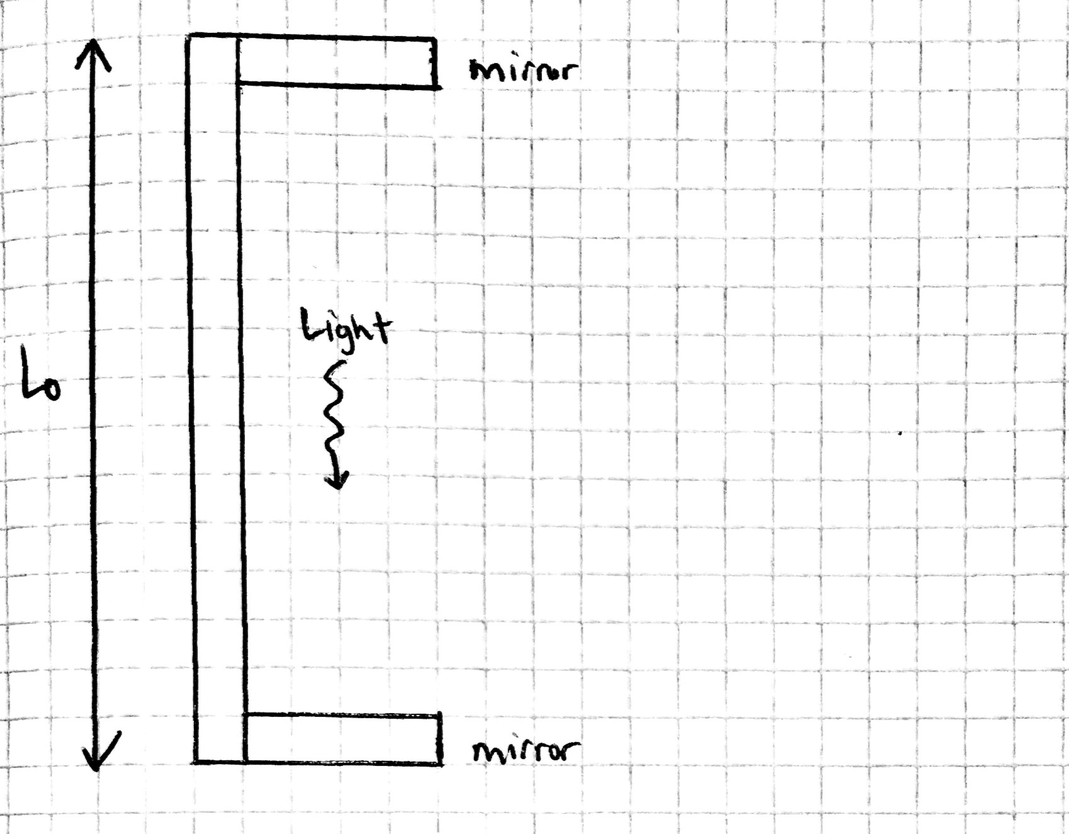
\includegraphics[width=100mm]{lightclock}\par
  \caption{Light Clock}
\end{figure}

\begin{figure}[!htb]
  \centering
  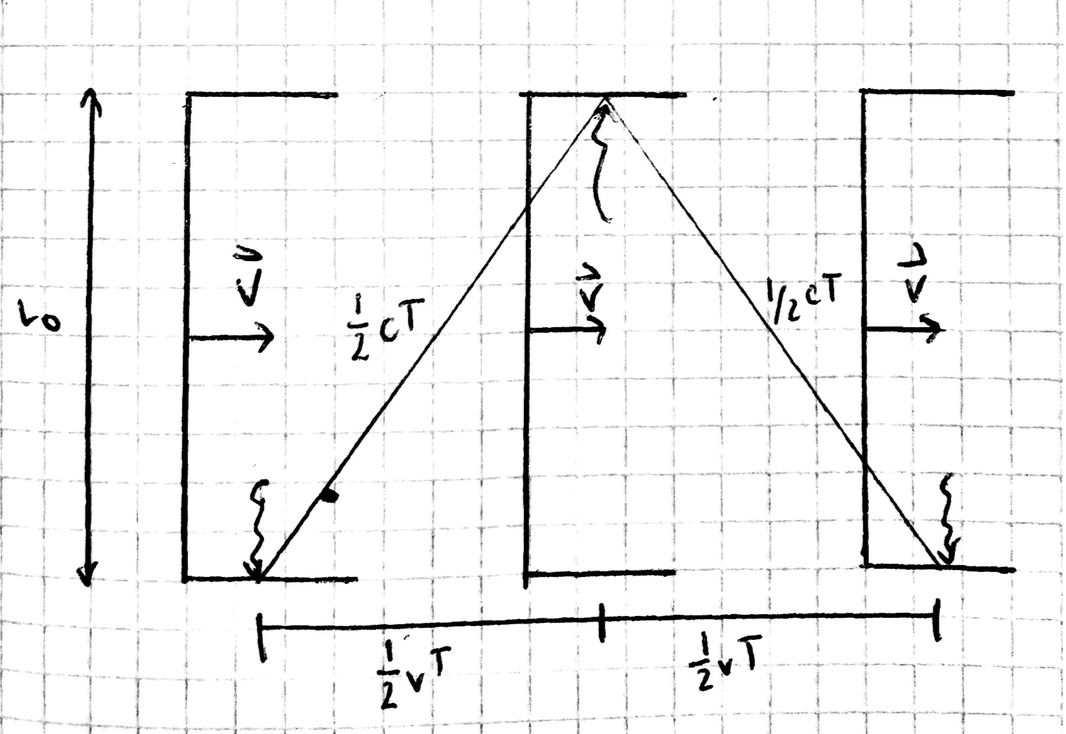
\includegraphics[width=100mm]{lightclockmoving}\par
  \caption{A Light Clock Moving with Velocity \(\vec{v}\)}
\end{figure}

\newpage
Suppose we construct a Light Clock, which is defined as the structure in Figure 1. The time between ticks \(T_0\) on a light clock is the time between when the light hits, say the lower mirror. Since the light travels a length \(L_0\), we can relate the time between ticks by \(2L_0 = cT_0\).

Consider when the light clock is moving at a velocity \(\vec(v)\). In this frame of reference, the clock moves a distance \(vT_0\) in between ticks, as demonstrated in Figure 2. Thus, the distance that the light is travelling by the Pythagorean theorem is now expressed as
\[
cT_0 = 2\sqrt{L_0^2 + (\frac{1}{2}vT_0)^2}
\]

But since we know that the speed of light is the same in all inertial frames, we can substitute in \(L_0 = \frac{1}{2}cT_0\) and you get
\[
cT_0 = 2\sqrt{(\frac{1}{2}cT_0)^2 + (\frac{1}{2}vT_0)^2}
\]

Solving for T yields
\[
  T = \frac{T_0}{\sqrt{1 - (\frac{\vec{v}^2}{c^2})}}
\]
\end{document}
